\documentclass[tikz,border=5pt]{standalone}
\usetikzlibrary{positioning}

\begin{document}
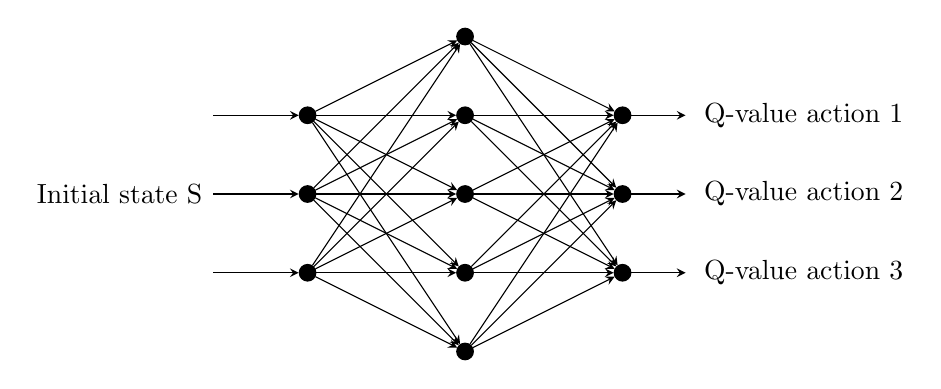
\begin{tikzpicture}[
    neuron/.style={circle, draw=black, fill=black, inner sep=0pt, minimum size=6pt},
    >=stealth
]

% Input layer (3 neurons)
\node[neuron] (I1) at (0,1) {};
\node[neuron] (I2) at (0,0) {};
\node[neuron] (I3) at (0,-1) {};
\node[left=1.1cm of I2] {Initial state S};

% Input arrows
\draw[->] (-1.2,1) -- (I1);
\draw[->] (-1.2,0) -- (I2);
\draw[->] (-1.2,-1) -- (I3);

% Hidden layer (5 neurons)
\node[neuron] (H1) at (2,2) {};
\node[neuron] (H2) at (2,1) {};
\node[neuron] (H3) at (2,0) {};
\node[neuron] (H4) at (2,-1) {};
\node[neuron] (H5) at (2,-2) {};

% Output layer (3 neurons)
\node[neuron] (O1) at (4,1) {};
\node[neuron] (O2) at (4,0) {};
\node[neuron] (O3) at (4,-1) {};

\node[right=0.8cm of O1] {Q-value action 1};
\node[right=0.8cm of O2] {Q-value action 2};
\node[right=0.8cm of O3] {Q-value action 3};

% Output arrows
\draw[->] (O1) -- ++(0.8,0);
\draw[->] (O2) -- ++(0.8,0);
\draw[->] (O3) -- ++(0.8,0);

% Connections: Input to Hidden
\foreach \i in {1,2,3}
  \foreach \h in {1,2,3,4,5}
    \draw[->] (I\i) -- (H\h);

% Connections: Hidden to Output
\foreach \h in {1,2,3,4,5}
  \foreach \o in {1,2,3}
    \draw[->] (H\h) -- (O\o);

\end{tikzpicture}
\end{document}
